% !TEX TS-program = XeLaTeX
% use the following command:
% all document files must be coded in UTF-8
\documentclass[spanish]{textolivre}
% build HTML with: make4ht -e build.lua -c textolivre.cfg -x -u article "fn-in,svg,pic-align"

\journalname{Texto Livre}
\thevolume{15}
%\thenumber{1} % old template
\theyear{2022}
\receiveddate{\DTMdisplaydate{2021}{11}{25}{-1}} % YYYY MM DD
\accepteddate{\DTMdisplaydate{2021}{12}{29}{-1}}
\publisheddate{\DTMdisplaydate{2022}{2}{10}{-1}}
\corrauthor{Viviana Guadalupe Azcorra Novelo}
\articledoi{10.35699/1983-3652.2022.37264}
%\articleid{NNNN} % if the article ID is not the last 5 numbers of its DOI, provide it using \articleid{} commmand
\runningauthor{Azcorra Novelo y Gallardo Córdova} 
\sectioneditorname{Leonardo C. Araújo}
\layouteditorname{Leonardo C. Araújo}

\title{Modelo de diseño de un instrumento para el aprendizaje y  evaluación adaptativa de saberes algebraicos}
\othertitle{Modelo para a concepção de um instrumento de aprendizagem adaptativa e avaliação do conhecimento algébrico}
\othertitle{Design model of an instrument for learning and adaptive assessment of algebraic knowledge}
% if there is a third language title, add here:
%\othertitle{Artikelvorlage zur Einreichung beim Texto Livre Journal}

\author[1]{Viviana Guadalupe Azcorra Novelo \orcid{0000-0001-6665-5016} \thanks{Email: \url{viviana.azcorra@correo.uady.mx}}}
\author[2]{Katherina Edith Gallardo Córdova \orcid{0000-0001-8343-9518} \thanks{Email: \url{katherina.gallardo@tec.mx}}}
\affil[1]{Universidad Autónoma de Yucatán, Facultad de Matemáticas, Yucatán, México}
\affil[2]{Instituto Tecnológico y de Estudios Superiores de Monterrey, Escuela de Humanidades y Educación, Monterrey, Nuevo León, México}

\addbibresource{article.bib}
% use biber instead of bibtex
% $ biber article

% used to create dummy text for the template file
%\definecolor{dark-gray}{gray}{0.35} % color used to display dummy texts
%\usepackage{lipsum}
%\SetLipsumParListSurrounders{\colorlet{oldcolor}{.}\color{dark-gray}}{\color{oldcolor}}

% used here only to provide the XeLaTeX and BibTeX logos
%\usepackage{hologo}

% if you use multirows in a table, include the multirow package
%\usepackage{multirow}

% provides sidewaysfigure environment
%\usepackage{rotating}

% CUSTOM EPIGRAPH - BEGIN 
%%% https://tex.stackexchange.com/questions/193178/specific-epigraph-style
%\usepackage{epigraph}
%\renewcommand\textflush{flushright}
%\makeatletter
%\newlength\epitextskip
%\pretocmd{\@epitext}{\em}{}{}
%\apptocmd{\@epitext}{\em}{}{}
%\patchcmd{\epigraph}{\@epitext{#1}\\}{\@epitext{#1}\\[\epitextskip]}{}{}
%\makeatother
%\setlength\epigraphrule{0pt}
%\setlength\epitextskip{0.5ex}
%\setlength\epigraphwidth{.7\textwidth}
% CUSTOM EPIGRAPH - END

% LANGUAGE - BEGIN
% ARABIC
% for languages that use special fonts, you must provide the typeface that will be used
% \setotherlanguage{arabic}
% \newfontfamily\arabicfont[Script=Arabic]{Amiri}
% \newfontfamily\arabicfontsf[Script=Arabic]{Amiri}
% \newfontfamily\arabicfonttt[Script=Arabic]{Amiri}
%
% in the article, to add arabic text use: \textlang{arabic}{ ... }
%
% RUSSIAN
% for russian text we also need to define fonts with support for Cyrillic script
% \usepackage{fontspec}
% \setotherlanguage{russian}
% \newfontfamily\cyrillicfont{Times New Roman}
% \newfontfamily\cyrillicfontsf{Times New Roman}[Script=Cyrillic]
% \newfontfamily\cyrillicfonttt{Times New Roman}[Script=Cyrillic]
%
% in the text use \begin{russian} ... \end{russian}
% LANGUAGE - END

% EMOJIS - BEGIN
% to use emoticons in your manuscript
% https://stackoverflow.com/questions/190145/how-to-insert-emoticons-in-latex/57076064
% using font Symbola, which has full support
% the font may be downloaded at:
% https://dn-works.com/ufas/
% add to preamble:
% \newfontfamily\Symbola{Symbola}
% in the text use:
% {\Symbola 😥}
% EMOJIS - END

% LABEL REFERENCE TO DESCRIPTIVE LIST - BEGIN
% reference itens in a descriptive list using their labels instead of numbers
% insert the code below in the preambule:
%\makeatletter
%\let\orgdescriptionlabel\descriptionlabel
%\renewcommand*{\descriptionlabel}[1]{%
%  \let\orglabel\label
%  \let\label\@gobble
%  \phantomsection
%  \edef\@currentlabel{#1\unskip}%
%  \let\label\orglabel
%  \orgdescriptionlabel{#1}%
%}
%\makeatother
%
% in your document, use as illustraded here:
%\begin{description}
%  \item[first\label{itm1}] this is only an example;
%  % ...  add more items
%\end{description}
% LABEL REFERENCE TO DESCRIPTIVE LIST - END


% add line numbers for submission
%\usepackage{lineno}
%\linenumbers

\begin{document}
\maketitle

\begin{polyabstract}
\begin{abstract}
El objetivo del presente estudio fue desarrollar una prueba desde el enfoque de aprendizaje adaptativo, que facilite realizar un diagnóstico que deriva en una trayectoria personalizada de actividades de aprendizaje para los estudiantes universitarios en función del nivel de dominio de las competencias para la materia de álgebra. Participaron 3 docentes en el diseño y se aplicó a 46 estudiantes universitarios. La prueba puntuó con una consistencia interna de 0.85. La aplicación permitió diseñar las trayectorias personalizadas con las que los estudiantes debían iniciar y progresar en su desempeño. Los resultados permiten indicar que las trayectorias personalizadas constituyen un apoyo esencial en la aplicación del aprendizaje adaptativo cuando se trabaja en modelos por competencias. 

%\keywords{palavra1 \sep palavra dois \sep palavra-três \sep palavra4}
\keywords{Álgebra \sep Aprendizaje adaptativo \sep Competencias \sep Educación superior \sep Evaluación adaptativa}
\end{abstract}

\begin{portuguese}
\begin{abstract}
O objetivo deste estudo é desenvolver um teste a partir da abordagem de aprendizagem adaptativa, que facilite um diagnóstico que resulte em uma trajetória personalizada de atividades de aprendizagem para estudantes universitários com base no nível de domínio das habilidades para a disciplina de álgebra. Três professores participaram do projeto e ele foi aplicado a 46 estudantes universitários. O teste obteve pontuação com consistência interna de 0,85. O aplicativo permitiu o desenho de trajetórias personalizadas com as quais os alunos tiveram que iniciar e progredir em seu desempenho. Os resultados permitem indicar que as trajetórias personalizadas constituem um suporte essencial na aplicação da aprendizagem adaptativa ao trabalhar em modelos baseados em competências. 

\keywords{Álgebra \sep Aprendizagem adaptativa \sep Competências \sep Ensino superior \sep Avaliação adaptativa}
\end{abstract}
\end{portuguese}

\begin{english}
\begin{abstract}
The objective of this study was to develop a test from the adaptive learning approach, which facilitates a diagnosis that leads to a personalized trajectory of learning activities for university students according to the level of mastery of the competencies for the subject of algebra. Three teachers participated in the design and it was applied to 46 university students. The test scored with an internal consistency of 0.85. The application made it  possible to design the personalized trajectories with which the students were to start and progress in their performance. The results indicate that personalized trajectories constitute an essential support in the application of adaptive learning when working in competency-based models.

\keywords{Algebra \sep Adaptive learning \sep Competencies \sep Higher education \sep Adaptive assessment}
\end{abstract}
\end{english}
% if there is another abstract, insert it here using the same scheme
\end{polyabstract}

\section{Introducción}\label{sec-intro}
Cada día alrededor del mundo, son más las instituciones educativas que están incorporando tecnologías emergentes como la Inteligencia Artificial, Aprendizaje Adaptativo y las Analíticas de Aprendizaje, por mencionar algunas. El objetivo es facilitar el acceso al conocimiento al estudiante en cualquier momento y lugar. Esto contribuye a ofrecer una educación flexible, dinámica y personalizada \cite{dziuban2016}. Por ejemplo, \textcite{sharma2019} proporcionaron una metodología para construir canales de aprendizaje automático para datos educativos multimodales. Con el objetivo de predecir el compromiso y desempeño del estudiante en entornos virtuales de aprendizaje adaptativo, utilizando Inteligencia Artificial y Aprendizaje Adaptativo. 

En este trabajo de investigación, el tema central es precisamente uno de los conceptos que ha conllevado al diseño de diferentes tecnologías emergentes: el Aprendizaje Adaptativo (AA). Este tiene una relación cercana al Aprendizaje Personalizado y al Aprendizaje Diferenciado. El primero consiste en estrategias que brindan soluciones e intervenciones que se ajustan a los objetivos individuales del estudiante. El segundo se caracteriza por ofrecer diferentes caminos para que el estudiante adquiera conocimiento con base en sus preferencias y estilo de aprendizaje. Por su parte, el AA utiliza un sistema por ordenador para crear una experiencia personalizada de aprendizaje y, así, lograr la adaptabilidad de la instrucción \cite{morillo2016}. %(LOZANO, 2016). 
Por tanto, el AA se considera una estrategia y también una herramienta para lograr el Aprendizaje Personalizado. 

Dicho lo anterior, se define al AA como un modelo, enfoque o técnica para crear experiencias de aprendizaje personalizado. Su objetivo es proporcionar rutas de aprendizaje eficientes, efectivas y personalizadas para cada estudiante. Emplea un enfoque sofisticado basado en datos, generalmente no lineal, para mejorar la instrucción, retroalimentación y corrección, puesto que se ajusta a las interacciones y al nivel de desempeño demostrado por el discente \textapud{partners2013}{murray2015} % PARTNERS (2013) 
y \textapud{moskal2017}{picciano2019}.

%conforme citado por \textcite{moskal2017}%; MOSKAL; CARTER; JOHNSON (2017) 
%conforme citado por \textcite{picciano2019}.

% Partners (2013 apud MURRAY; PÉREZ, 2015) y Moskal; Carter; Johnson (2017 apud PICCIANO, 2019)

Se sabe que existen posturas complementarias que integran elementos de diferentes fuentes disciplinarias al AA. Al inicio, el AA estuvo influenciado por los avances de varias disciplinas. Por ejemplo, \cite{virgili2018} %(TORRAS, 2018) 
indica que este concepto tiene una naturaleza multidisciplinar. De hecho, es un constructo que se relaciona con las ciencias de la educación, la inteligencia artificial, la psicología y la neurociencia. Las más importantes son la psicología educativa, tecnología educativa y la neurociencia. Por tanto, para efectos de esta investigación, la descripción de su evolución se estructurará en dos temáticas, tecnologías para la educación y cómo aprende el ser humano.  

\textcite{picciano2019} afirma que el AA tiene sus inicios con las aproximaciones de la Instrucción Asistida por Computadora (CAI) y la máquina de enseñanza de Skinner. En 1959 y 1970 surge el Programmed Logic for Automated Teaching Operations (PLATO) y el primer Sistema Tutorial Inteligente denominado SCHOLAR (por el MIT), respectivamente. Los cuales contribuyeron a automatizar la instrucción individualizada y anticipar las respuestas de quien aprende. No obstante, desde el año 2000 con el surgimiento de los Sistemas de Gestión del Aprendizaje (LMS, por sus siglas en inglés) se detonó el desarrollo y crecimiento de los sistemas computacionales, la Inteligencia Artificial y las Analíticas de Aprendizaje, las cuales comenzaron a tener impacto en el AA. Actualmente, se cuentan con plataformas específicas para el AA, como, por ejemplo: Smart Sparrow (\url{https://www.smartsparrow.com/}), Knewton (\url{https://www.knewton.com/}), Cogbooks (\url{https://www.cogbooks.com/}), entre otras. 

\begin{table}[h!]
\caption{Características de las teorías de aprendizaje que sustentan el aprendizaje adaptativo} % title of Table
\centering % used for centering table
\begin{tabular} { c      p{8cm}  p{4cm} } % centered columns (2 columns)
\hline %inserts double horizontal lines
Teorías & Características \\ [0.4ex] % inserts table
%heading
\hline % inserts single horizontal line
Conductista & \begin{itemize}
    \item Pavlov desarrolló el paradigma clásico
    \item Thorndike desarrolló el paradigma experimental
    \item Skinner contribuyó al condicionamiento particular y al conductismo en general
\end{itemize} \\ % inserting body of the table
Cognitivismo & \begin{itemize}
    \item Los procesos constructivos tienen su origen en la toma de conciencia de los desajustes entre las representaciones mentales de los alumnos y la realidad de la que pretende dar cuenta
\end{itemize} \\
Socioconstructivismo & \begin{itemize}
    \item Los procesos son más equilibrados y enfatiza la importancia del papel del entorno social y el entorno físico en la construcción del conocimiento
\end{itemize} \\
\hline %inserts single line
\end{tabular}
\label{tbl01} % is used to refer this table in the text
\source{\cite{lau2016}}
\end{table}

Si bien el AA no puede desvincularse teóricamente del aprendizaje y sus diferentes enfoques, tales como el conductismo, cognitivismo o el socioconstructivismo, éstas sitúan al aprendiz en un lugar central, de modo que la personalización del aprendizaje está presente en estos paradigmas clásicos. Por tanto,
Povlov, Thorndike, Piaget y Vigostky, se consideran los
principales referentes de dichas teorías (ver \Cref{tbl01}). Puesto que tuvieron como objeto de estudio los mecanismos de adaptación del organismo al entorno, siendo el aprendizaje un elemento clave en esta adaptación.

En cuanto al AA y su relación con la evaluación del aprendizaje, es pertinente indicar que existe una codependencia entre ambos constructos. Se sabe que la evaluación del aprendizaje, relacionada con el AA, enfoca sus prácticas en lograr la medición del progreso del estudiante y, con ello, precisar o mejorar la instrucción personalizada, se denomina Evaluación Adaptativa (EA) \cite{edutrends2014}.%(LEMKE, 2014). 
Dicho lo anterior, para fines de esta investigación, se considerará a la EA como parte inherente del AA. Sus características se observan en la \Cref{fig:01} y su relación en la \Cref{fig:02}.

\begin{figure}[h!]
   \centering
   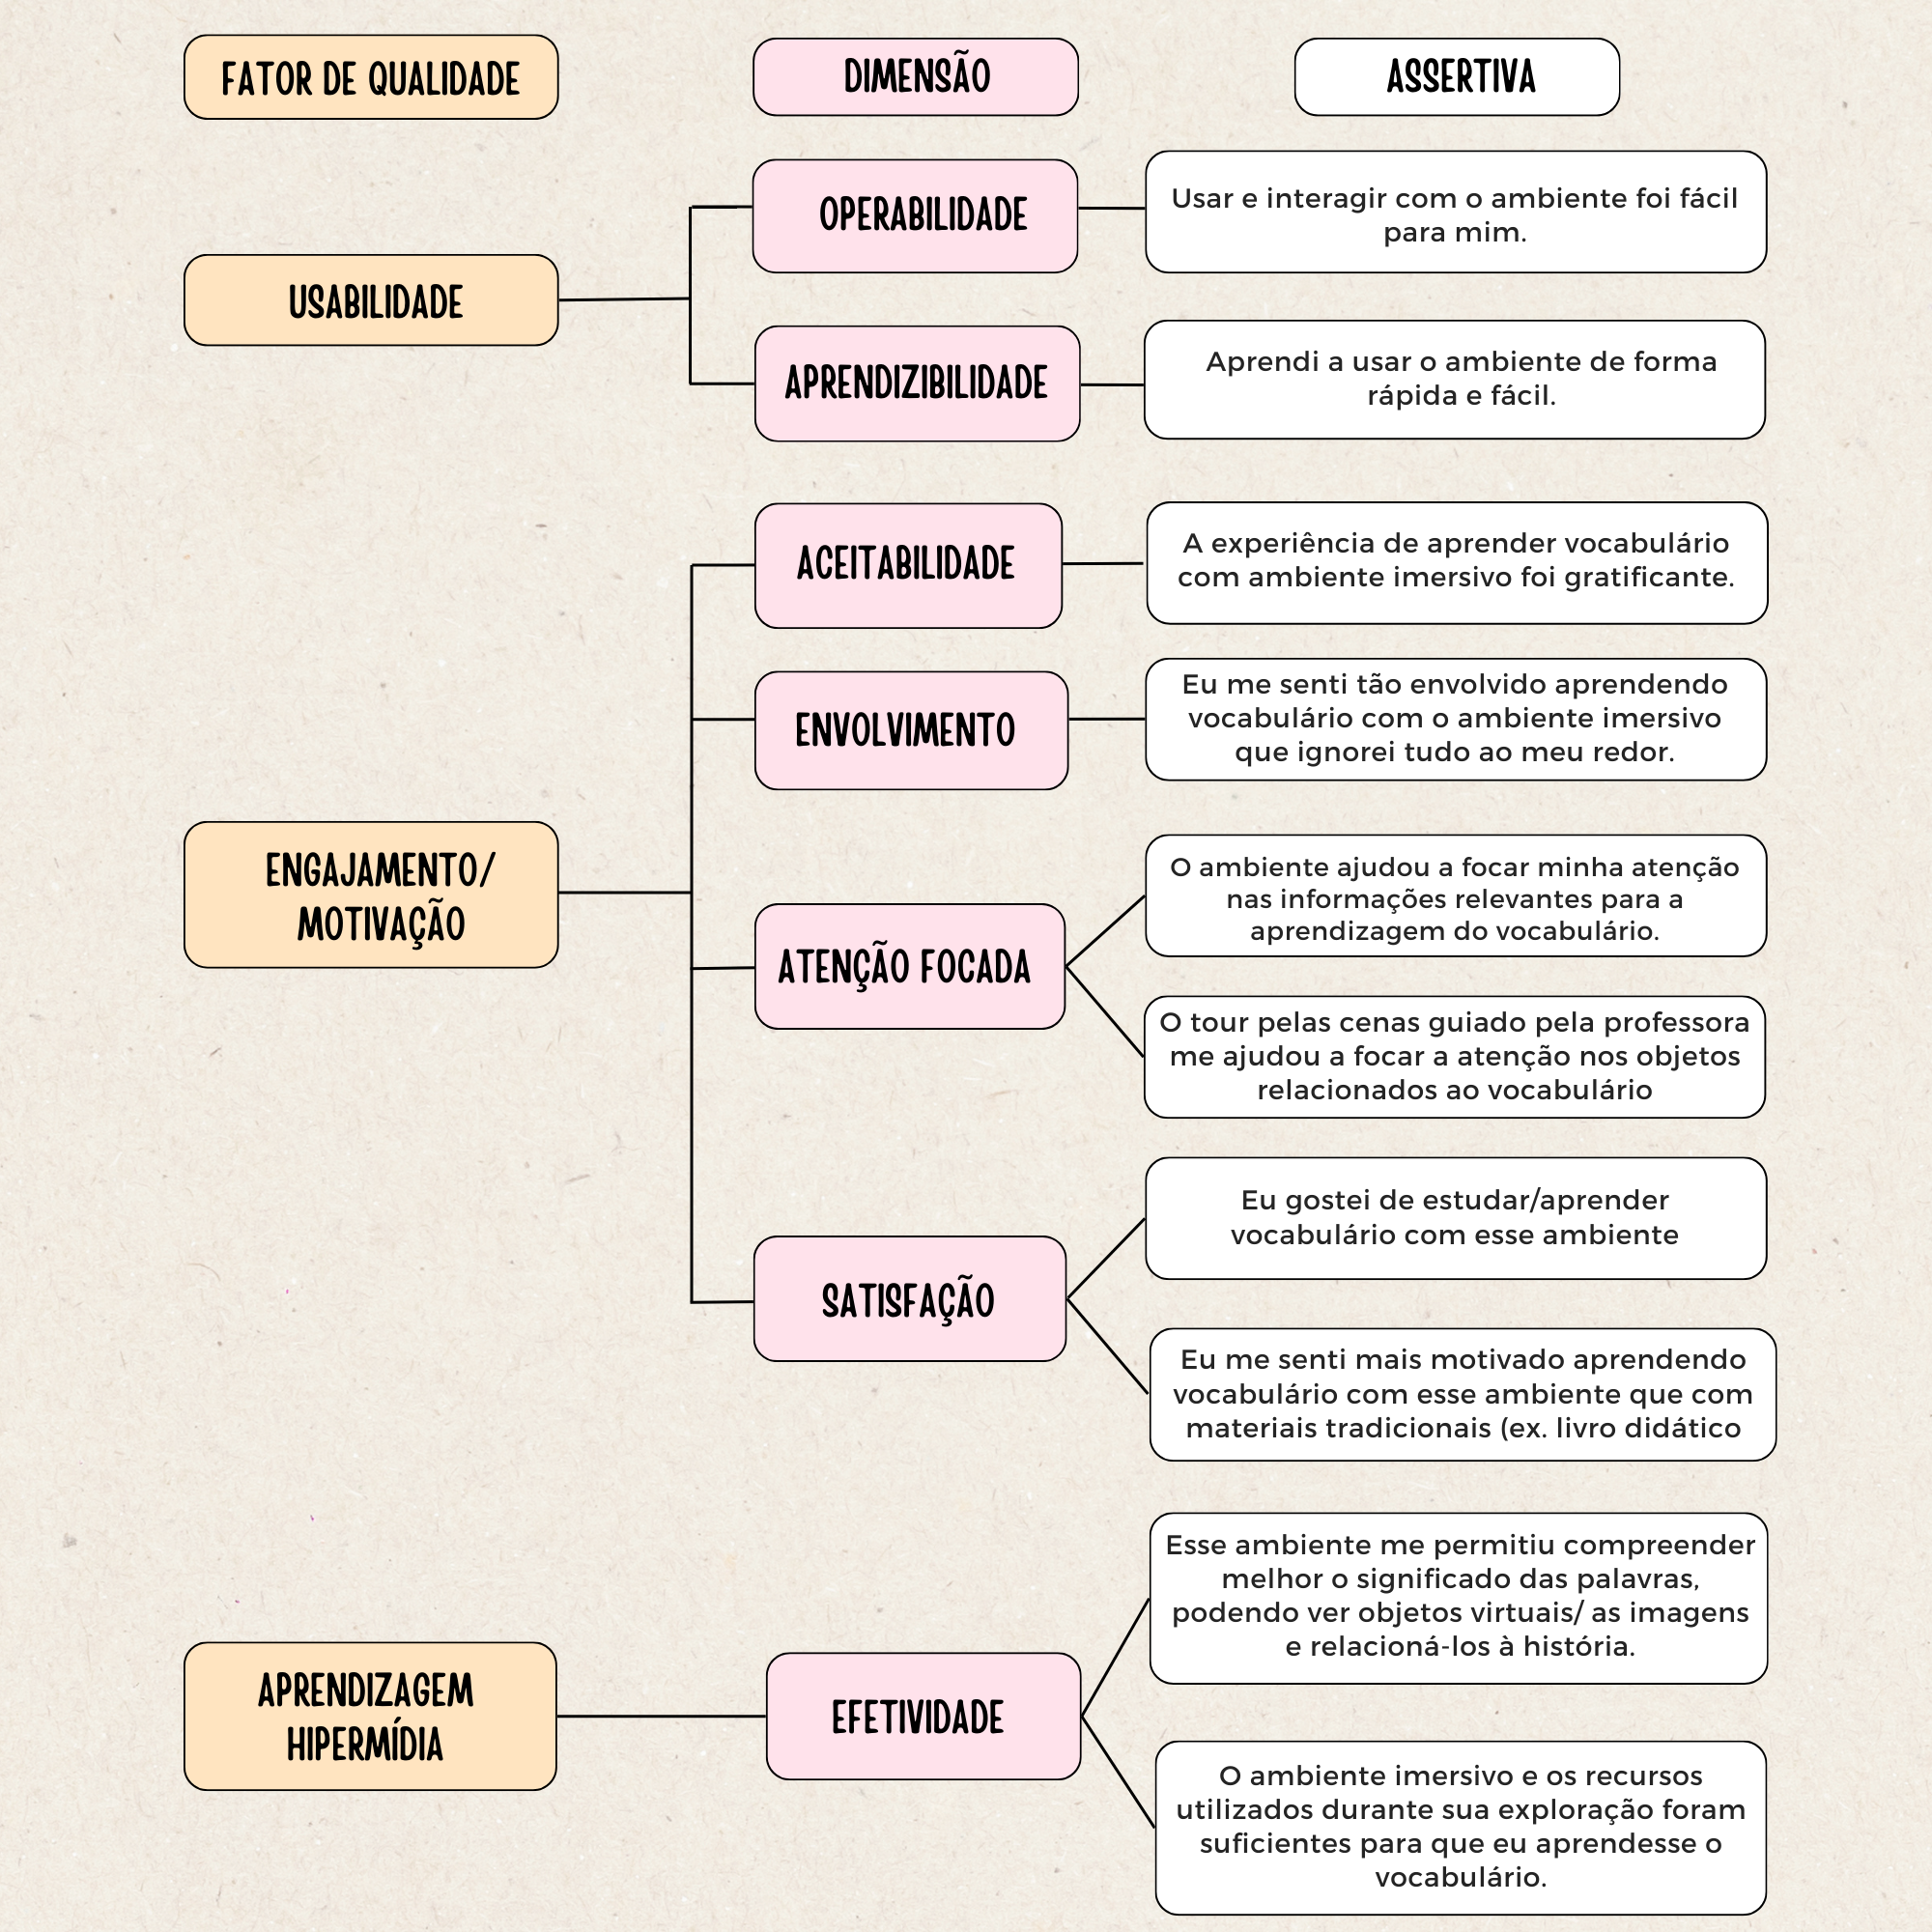
\includegraphics[width=\textwidth]{fig-01.pdf}
   \caption{Relación del Aprendizaje Adaptativo y la Evaluación Adaptativa.}
   \source{Elaboración propia.}
   \label{fig:01}
\end{figure}

\begin{figure}[h!]
   \centering
   \includegraphics[width=\textwidth]{fig-02.pdf}
   \caption{Vista adaptativa para el tratamiento y emisión de trayectorias.}
   \source{Elaboración propia.}
   \label{fig:02}
\end{figure} 

Es importante indicar que en esta investigación el punto medular de interés conlleva abordar la función pedagógica de la evaluación, la cual se vincula con la evaluación continua realizada por el docente. Con el fin de valorar si el alumno ha adquirido las competencias planteadas o logrado los aprendizajes esperados \cite{inee2019}. %(INEE, 2017). 
\textcite{black2018}B %LACK; WILIAM (2018) 
afirman que este proceso puede desarrollarse con base en tres enfoques. Evaluación del aprendizaje (assessment of learning), el cual se interesa en determinar el grado de asimilación de los contenidos del curso por el estudiante. Mientras que la evaluación para el aprendizaje (assessment for learning) busca ser parte fundamental del proceso de enseñanza y aprendizaje, es decir, que los mecanismos que se utilicen sean de utilidad tanto para el profesor como al alumno \textcite{scriven1967} %SCRIVEN (1967) 
conforme citado por \textcite{taras2005}. Finalmente, la evaluación como aprendizaje (assessment as learning) favorece a que el discente aprenda mientras es evaluado.

Aunado a lo anterior, en las investigaciones de \textcite{taras2005,taras2008,lau2016} %TARAS (2005, 2008) y MAN; LAU (2015) 
se hace hincapié en el establecimiento sinérgico de las intenciones de la evaluación. Esto quiere decir que, si bien la evaluación está matizada con base en algún enfoque, los juicios que realice el profesor deberán regirse con base en las intenciones evaluativas. Las cuales se caracterizan por tener una naturaleza distinta entre sí y, a su vez, se complementan para coadyuvar en la toma de decisiones del educador durante la instrucción y en el aprendizaje del discente.

Por tanto, \textcite{taras2005} afirma que la evaluación sumativa y formativa se relacionan entre sí. En este sentido, si bien la evaluación es un proceso único que se apoya de una o varias intenciones, \textcite{taras2005,sadler1989} conforme citado por \textcite{taras2005} sostienen que primero es necesario evaluar la calidad del trabajo antes de que el alumno pueda utilizar la retroalimentación. Es decir, no es posible que la evaluación sea únicamente formativa sin que se emita un juicio sumativo. Por tanto, \textcite{black2018} afirman que ambas intenciones de evaluación pueden usar el mismo instrumento de evaluación y los resultados para realizar juicios y retroalimentaciones según sea el caso. Por tanto, la única diferencia entre dichas intenciones recae en los tipos de inferencias que se extraen sobre la base de los resultados de aprendizaje.

En cuanto a la intención diagnóstica de la evaluación, si bien no existe una definición universal, varios autores que la han caracterizado \cite{csapo2019}. Por tanto, se dice que una evaluación tiene una intención diagnóstica cuando se realizan juicios o inferencias que encapsulan toda la evidencia respecto al conocimiento, habilidades y actitudes que posee el estudiante antes de iniciar un curso o unidad de aprendizaje, mediante el uso de una variedad de métodos y herramientas \cite{javidanmehr2017,tangeokshim2017}.

\textbf{El estudiante universitario.} En cuanto a las características de la población de este estudio, resulta necesario partir de la definición de la Andragogía. Según \textcite{castro1990} conforme citado por \textcite[p.~69]{castillo2018} es (…) “"una de las Ciencias de la Educación que tiene por finalidad facilitar los procesos de aprendizaje en el adulto a lo largo de toda su vida"”. La principal diferencia respecto a la Pedagogía es que en ésta existe un proceso de Enseñanza-Aprendizaje, mientras que en la Andragogía se promueve un proceso de Orientación-Aprendizaje. Esto implica que el aprendiz adulto construye su aprendizaje y, el facilitador, atiende y orienta a los participantes para que puedan asegurar sus aprendizajes. 

\textcite{knowles2006} conforme citado por \textcite[p.~65]{castillo2018} afirma que ""para definir el término aprendiz adulto resulta importante considerar cuatro áreas: biológica, legal, social y psicológica"". No obstante, para determinar cuándo el alumno debe ser tratado como adulto, \textcite{knowles1980} conforme citado por \textcite{domenech2015} %SÁNCHEZ (2015) 
responde a dos de las cuatro áreas, la social y la psicológica. De acuerdo con \textcite{domenech2015}, las características del estudiante adulto se articulan con los supuestos o principios andragógicos, los cuales son a) la necesidad de saber, b) el autoconcepto del alumno, c) el papel de la experiencia, d) la disposición para aprender, e) la orientación al aprendizaje y f) la motivación. 

Como se ha visto, en el área educativa surgen constantemente nuevas prácticas para favorecer y promover el aprendizaje. Así como tecnologías emergentes que coadyuvan en la resolución de necesidades en la educación, tanto en ámbitos presenciales como a distancia. El AA es una de las tecnologías educativas que actualmente se sitúa en la curva ascendente en el Hype Cycle for Emerging Technologies del 2011, gracias a su uso y los beneficios que ofrece en los procesos de enseñanza y aprendizaje \cite{brown2020}. %(BROWN et al., 2020). 
No obstante, resulta necesario generar estudios para vislumbrar cómo mejoran el rendimiento de los estudiantes y reducen las brechas de aprendizaje en diferentes contextos.

\textcite{anderson2019,dziuban2017,dziuban2016,feldman2017,educause2019}
%ANDERSON (2019), DZIUBAN, CHARLES et al. (2017), DZIUBAN, CHARLES D et al. (2016), ESSA; LASTER (2017) y ALEXANDER et al. (2019) 
afirman que el uso del AA en la educación superior es un área emergente de estudio. Ya que todavía hay evidencia limitada sobre cómo los sistemas adaptativos mejoran el rendimiento de los estudiantes y reducen las brechas de aprendizaje. \textcite{boyce2020} mencionan que, en los cursos de matemáticas a nivel superior, es necesario integrar herramientas de AA junto con el aprendizaje activo para favorecer el aprendizaje procedimental y conceptual de saberes matemáticos. Para ello, resulta necesario recurrir a la andragogía, puesto que contribuye en el proceso de aprendizaje de un adulto. Asimismo, favorece la adaptación de alumnos adultos a un lugar de trabajo en constante cambio \cite{cretchley2001,merriam2001}.

Luego de lo anteriormente expuesto, se planteó la necesidad de responder a través de una investigación de qué manera una prueba diseñada desde el enfoque de aprendizaje adaptativo facilita realizar un diagnóstico, que permita delinear trayectorias personalizadas de aprendizaje. Para efectos de este estudio, el proceso de aprendizaje y evaluación adaptativos se realizó alrededor de las competencias de álgebra para estudiantes de educación superior de diversas disciplinas.

\section{Método}\label{sec-normas}
Esta investigación se realizó desde un enfoque de estudio exploratorio \textcite{gonzalez2014}. La investigación se circunscribe en una institución de educación superior del sur de México. En esta se ofrecen programas educativos del área de ciencias exactas. En el primer semestre se ofertan asignaturas para nivelar los conocimientos básicos, como es el caso de álgebra intermedia. Si algún estudiante no lo aprueba, en el siguiente semestre se oferta la asignatura en la modalidad por acompañamiento o repetición del curso. En ambos, se aplica un diagnóstico para ubicar al estudiante en los contenidos que le faltan precisar.

\subsection{Participantes}\label{sec-conduta}
En esta investigación participaron tres profesores expertos en Matemáticas y 46 estudiantes con atributos particulares: estar inscritos en el curso de álgebra intermedia por acompañamiento (20) o repetición del curso (26) de los programas de estudio de Licenciatura en Actuaría, Licenciatura en Ciencias de las Computación, Licenciatura en Ingeniería de Software, Licenciatura en Ciencias de la Computación y Licenciatura en Enseñanza de las Matemáticas.

\subsection{Instrumentos}\label{sec-fmt-manuscrito}
El objetivo de la investigación se centró en el desarrollo y aplicación un instrumento diagnóstico, por medio de la herramienta lección de MOODLE, para conocer las fortalezas y áreas de oportunidad de los estudiantes desde la evaluación adaptativa \cite{dziuban2017,dziuban2016}. 

Para el desarrollo del examen diagnóstico de álgebra, se tomó como base la Nueva taxonomía \cite{marzano2008}, la planeación didáctica del curso de álgebra intermedia, así como el desagregado de niveles de dificultad. Respecto al nivel taxonómico, \textcite{marzano2008} describen al Dominio de Conocimiento (DC) como aquello que hace alusión al proceso de pensamiento que permite su aprendizaje, y se divide de la siguiente manera (p.~9):

\begin{itemize}
\item Información. En la base de la jerarquía de este primer tipo de conocimiento están ubicadas las palabras que conforman el nivel denominado vocabulario, hechos, secuencias de eventos, generalizaciones o principios.
\item Procedimientos mentales. Es también conocido como conocimientos procedimentales que se logran atender mediante un proceso de memorización y familiarización que emana de la experiencia. Este se subdivide en reglas simples, algoritmos, tácticas y macroprocedimientos.
\end{itemize}

En cuanto a los Niveles de Procesamiento (NP) está conformado por los tres sistemas: self, metacognitivo y cognitivo. En particular, el sistema cognitivo tiene los niveles (p.~4 y 5):

\begin{itemize}
\item Nivel 1 Recuperación. Activación y transferencia del conocimiento de la memoria permanente a la memoria del trabajo, donde se puede ser conscientemente procesada. Los procesos que conforman la recuperación son: reconocimiento y recuerdo o ejecución. 
\item Nivel 2 Comprensión. Es el encargado de traducir el conocimiento en las formas adecuadas para que su almacenaje en la memoria permanente se produzca. Los procesos que conforman la comprensión son integración y simbolización.
\item Nivel 3 Análisis. Corresponde a la extensión razonada del conocimiento y va más allá de la identificación de lo esencial y lo no esencial, que son funciones propias de la comprensión. Los procesos que conforman el análisis son asociación, clasificación, detención del error, generalización y especificación.
\item Nivel 4 Utilización del conocimiento. Este se presenta cuando la persona se ve en la necesidad de cumplir con determinadas tareas y, estas, se pueden considerar como las avenidas por donde corre el conocimiento. Está conformado por cuatro categorías, la toma de decisiones, resolución de problemas, experimentación e investigación.
\end{itemize}

Estos niveles que enuncia la Nueva taxonomía \cite{marzano2008} permitieron clasificar las preguntas de acuerdo con el nivel de desempeño y analizar las diferentes trayectorias que subyacen de la vista adaptativa, combinando el nivel taxonómico y de dificultad para cada unidad. Para efectos de emitir un resultado sobre el alcance en el desarrollo de las competencias, se determinaron a priori los siguientes escenarios: 

\begin{enumerate}
    \item El estudiante responde correctamente todas las opciones (respuesta y procedimiento). De ser así, un ítem se omite o varios se omiten, de acuerdo con la ruta crítica establecida (ver la primera opción de la tabla). 
\item El estudiante responde erróneamente (tanto la opción correcta como el procedimiento) todas las opciones. En este caso, responde todos los reactivos, incluyendo los que no están en la ruta crítica.  
\item El estudiante responde, de manera aleatoria, correcta e incorrectamente las opciones. En este caso, de igual manera responde todos los ítems de la prueba diagnóstica. 
\end{enumerate}

\subsection{Procedimientos y estrategias de análisis}\label{sec-formato}
La recolección y procesamiento de datos involucra un estudio distribuido en cuatro fases:

\begin{enumerate}
    \item Desarrollo del diagnóstico, las rutas críticas y solicitud de permiso a la institución para la participación de profesores y estudiantes. 
\item Convocatoria a estudiantes y profesores a participar en la evaluación de los reactivos y el pilotaje del diagnóstico.
\item Aplicación del diagnóstico en tres cursos de la asignatura de Álgebra Intermedia. Estos se conforman por dos grupos de repetición de curso y un grupo por acompañamiento. Se califican los resultados y se establecen las rutas de aprendizaje para cada estudiante. Para efectos de esta investigación, se eligieron dos grupos de estudiantes, conformados por cinco con calificación alta y cinco con calificación baja. 
\item Dar a conocer a los estudiantes sus resultados del diagnóstico y las rutas de aprendizaje personalizadas. Además, se realizan las entrevistas con profesores y estudiantes.
\end{enumerate}

\section{Resultados}\label{sec-modelo}
Para el desarrollo de la prueba diagnóstica se consideraron tres elementos: la planeación didáctica de la asignatura de álgebra intermedia, la taxonomía de \textcite{marzano2008} y los niveles de dificultad establecidos por la academia de álgebra (nivel 1, 2 y 3). Se revisó por unidad, las competencias y los resultados de aprendizaje  \footnote{El resultado de aprendizaje es una competencia de menor nivel y precisa en cierta contenido. Competencia \cite{uady2012}:%(UADY, 2012): 
es la integración dinámica de conocimientos, habilidades, actitudes y valores que permitan al egresado desempeñarse como ciudadano autónomo y flexible en una función, actividad o tarea profesional o social, a lo largo de la vida.}  para cada contenido. A continuación, se comparten ejemplos de tres reactivos, uno por cada nivel de dificultad y resaltando los tres elementos descritos con anterioridad.

En las Tablas se comparten tres reactivos de la Unidad II, los cuales corresponden al resultado de aprendizaje realizar correctamente operaciones con expresiones racionales. Por lo que, para medirlo, se consideraron cuatro reactivos de nivel 1, los cuales corresponden a simplificación, multiplicación, división y suma-resta de expresiones racionales. Mientras que, para los niveles 2 y 3, un reactivo para cada uno. De tal manera que, para el nivel 2, se favorecen aspectos conceptuales de las expresiones racionales y, para el nivel 3, un problema en el cual la expresión racional está implícita. Finalmente, las opciones de respuestas se diseñaron considerando las respuestas de estudiantes de cursos pasados.

En la \cref{tbl02} se presenta un ejercicio de simplificación de expresiones racionales (sencillas), el cual corresponde a una instrucción directa y solo requiere de cálculos sencillos (nivel 1). Por tanto, el estudiante tendrá que utilizar cierta información o principios, así como de reglas simples (dominios del conocimiento), para el recuerdo o ejecución (niveles de procesamiento) de procedimientos.

\begin{table}[h!]
\caption{Reactivo 1 de la Unidad II y de nivel 1} % title of Table
\centering % used for centering table
\begin{tabular} { c p{4cm} p{9cm} } % centered columns (2 columns)
\hline %inserts double horizontal lines
\#1 & Base de la pregunta &El resultado de simplificar la expresión$\frac{(x+6)(x-3)+(x+6)(x-2)}{2(x+6)}$ \\ [0.4ex] % inserts table%heading
\hline % inserts single horizontal line
A.  & Opción correcta &$\frac{2x-5}{2}$\\% ieting body of the table
b. & Distractor 1 & $x-5$ \\
C. & Distractor 2 & $x^2+3x-18$\\
D. & Distractor 3  & $\frac{x^2}{2}+2x-10$\\
. & Justificación 1 & Error al cancelar el número $2$\\
. & Justificación 2 & Error al cancelar el $(x+6)$ sin haber factorizado antes y después el $-2$ con el $2$ del denominador\\
. & Justificación 3 & Error al cancelar el $(x+6)$ sin haber factorizado antes\\
. & Nivel taxonómico & D.C. A.5 y NP 1.2\\
\hline
\end{tabular}
\label{tbl02} % is used to refer this table in the text
\source{Elaboración propia.}
\end{table}

En la \Cref{tbl03} se comparte un ejercicio que involucra monomios con exponentes literales para obtener el grado absoluto y el coeficiente, por lo que, corresponde a la resolución de uno o más operaciones, aplicando propiedades y definiciones (nivel 2). Por tanto, el estudiante tendrá que utilizar cierta información o principios, así como algoritmos (dominios del conocimiento), para el recuerdo o ejecución (niveles de procesamiento) de ciertos procedimientos.

\begin{table}[h!]
\caption{Reactivo 5 de la Unidad II y de nivel 2} % title of Table
\centering % used for centering table
\begin{tabular} { c p{4cm} p{9cm} } % centered columns (2 columns)
\hline %inserts double horizontal lines
\#5 & Base de la pregunta & El grado absoluto y el coeficiente de la simplificación de la expresión $\frac{[(x^2y)^{2n+1}][70(x^2y)^{2n}][10(x^2y)^{2n+5}][10(x^2y)^n]}{35(x^2y)^{7n+1}}$, donde $n \in Z^{+}$, es: \\ [0.4ex] % inserts table%heading
\hline % inserts single horizontal line
A.  & Opción correcta &$\frac{2x-5}{2}$\\% ieting body of the table
b. & Distractor 1 & $x-5$ \\
C. & Distractor 2 & $x^2+3x-18$\\
D. & Distractor 3 & Grado absoluto: $-n-5$ y coeficiente: $200$\\
. & Justificación 1 & Error al determinar el grado absoluto del monomio resultante \\
. & Justificación 2 & A pesar de la nota, se sumaron los coeficientes de los monomios \\
. & Justificación 3 & No se sumaron todos los exponentes \\
. & Nivel taxonómico & D.C. A.5 y B.2 / NP 1.2\\
\hline
\end{tabular}
\label{tbl03} % is used to refer this table in the text
\source{Elaboración propia.}
\end{table}

En la \Cref{tbl04} se tiene un problema intramatemático que involucra varios aspectos conceptuales y procedimentales de la Unidad I y II, por lo que, se requiere la comprensión del problema y el uso de conocimientos previos (nivel 3). Por tanto, el estudiante tendrá que utilizar macro procedimientos (dominios del conocimiento), para la resolución de problemas (niveles de procesamiento). 

\begin{table}[h!]
\caption{Reactivo 6 de la Unidad II y de nivel 3} % title of Table
\centering % used for centering table
\begin{tabular} { c p{4cm} p{9cm} } % centered columns (2 columns)
\hline %inserts double horizontal lines
\#6 & Base de la pregunta & Si $(x-a)$ y $(x-b)$, donde $a$ y $b$ no son iguales a CERO, son factores de $x^2+8x+15=0$. Selecciona la opción que indique el valor de $a$ y $b$, así como de la expresión $a^2+b^2+12ab$. \\ [0.4ex] % inserts table%heading
\hline % inserts single horizontal line
A.  & Opción correcta &$a=-5$y $b=-3$, el valor de la expresión es $214$\\
B.  & Distractor 1 &$a=-5$y $b=-3$, el valor de la expresión es $164$ \\
C. & Distractor 2  &$a=5$y $b=3$, el valor de la expresión es $214$ \\
D. & Distractor 3  &$a=5$y $b=3$, el valor de la expresión es $196$ \\
. & Justificación 1 & Factorizó adecuadamente, pero no aplicó correctamente las leyes de los exponentes\\
. & Justificación 2 & Factorizó adecuadamente, pero tuvo un error de signo en el despeje\\
. & Justificación 3 & Factorizó bien, pero tuvo error de signo en el despeje y no aplicó correctamente las leyes de los singos\\
. & Nivel taxonómico & D.C. B.4/NP 4.2\\
\hline
\end{tabular}
\label{tbl04} % is used to refer this table in the text
\source{Elaboración propia.}
\end{table}

Después de diseñar todos los reactivos para cada unidad, se creó la ruta crítica, con diferentes posibles escenarios (ver tabla de trayectorias). La cual tiene como intención plantear una vista adaptativa para el tratamiento y emisión de trayectorias y, con ello, emitir un resultado sobre el alcance en el desarrollo de competencias por parte de los estudiantes (ver \Cref{fig:03}). Por tanto, se eligieron reactivos de diferentes niveles de dificultad, pero dada la competencia de la asignatura, estos fueron más de nivel 1 y 2. Mientras que, los reactivos de nivel 3, se usaron para identificar a los estudiantes que tengan un nivel de dominio superior.

Cabe recalcar que se identificaron ejercicios que requerían mayor especificidad para lograr identificar las áreas de oportunidad y las habilidades que sí dominan los estudiantes. Esto únicamente ocurrió en la Unidad I, específicamente en los reactivos del uno al cuatro y el sexto. Puesto que se involucran operaciones o definiciones de cursos básicos que, incluso, podrían nublar el juicio del profesor al momento de crear la trayectoria de aprendizaje personalizada. Es por ello por lo que se presentarán resultados con distintas intencionalidades. Por un lado, para efectos de la trayectoria o ruta de aprendizaje, se incluyeron los resultados obtenidos en los reactivos adicionales de la Unidad I y, por otro lado, para efectos del análisis psicométrico, se consideró la prueba diagnóstica sin dichos reactivos adicionales.

\subsection{Resultados del análisis del diagnóstico y las trayectorias de aprendizaje.}\label{sec-organizacao-latex}

Es preciso recalcar que, dado que no se encontró algún sistema de aprendizaje adaptativo centrado en competencias, se utilizó la herramienta lección de MOODLE para programar la prueba diagnóstica, ya que permite un enfoque de adaptabilidad en los reactivos, aunque su principal función no es esta. De los 46 estudiantes que conformaron la muestra, únicamente 27 presentaron la prueba diagnóstica y la terminaron. Por tanto, para el análisis de los resultados del diagnóstico y la trayectoria de aprendizaje personalizada, se seleccionó un grupo de 10 estudiantes, de tal forma que, cinco tengan la calificación más alta y, los otros cinco, la calificación más baja. De dicho grupo se obtuvieron los siguientes resultados (ver \Cref{fig:03}).

\begin{figure}[h!]
   \centering
   \includegraphics[width=0.85\textwidth]{fig-03.pdf}
   \caption{Resultados del grupo de diez estudiantes, en la prueba diagnóstica.}
   \source{Elaboración propia.}
   \label{fig:03}
\end{figure}

La calificación más alta, en la escala de 0 a 100, es de 76 (51 respuestas correctas) y la más baja de 24 (16 respuestas correctas). La moda fue 67, lo que equivale a 45 reactivos contestados de manera correcta. No obstante, en cuanto al promedio de las calificaciones y el dato central del grupo, se tiene una cantidad muy similar, siendo 53 y 54; la cual equivale a tener entre 29 y 43 reactivos correctos. Posteriormente a la determinación de las calificaciones, se procedió a desarrollar manualmente las trayectorias de aprendizaje personalizadas \textapud{partners2013}{murray2015};
\textapud{moskal2017}{picciano2019},
%\textcite{partners2013} % Partners (2013) 
%conforme citado por \textcite{murray2015,carter2017} %MURRAY; PÉREZ (2015); Carter y Johnson (2017) 
%conforme citado por \textcite{picciano2019}, 
teniendo como eje central el logro de las competencias y resultados de aprendizajes. 

Del proceso que se llevó a cabo para desarrollar las trayectorias de aprendizaje personalizadas, es preciso recalcar que resultó necesario organizar cada unidad por resultados de aprendizaje y, estos a su vez, por reactivos que corresponden a cada una, resaltando la ruta crítica por colores según el nivel de dificultad (ver \Cref{fig:04}). Esto ayudó a identificar con mayor facilidad las competencias que se dominan y las que no. 

\begin{figure}[h!]
   \centering
   \includegraphics[width=1\textwidth]{fig-04.pdf}
   \caption{Unidad I organizada por resultados de aprendizaje y ruta crítica.}
   \source{Elaboración propia.}
   \label{fig:04}
\end{figure}

Para decidir las competencias que sí se lograron, se consideró el cumplimiento de la ruta crítica (los colores rojo, amarillo y verde); cabe recalcar que dichas competencias se consideraban logradas desde que cumplan con el nivel 1 (rojo), nivel 1 y nivel 2 (amarillo) o con los tres niveles. De lo contrario, para no errar, se revisaron los reactivos que no corresponden a la ruta crítica (por ejemplo, P5, P13 y P15) y los procedimientos desarrollados en cada reactivo. Por ejemplo, el caso del último renglón de la (tabla de excel), se observa que se tuvo incorrecto el reactivo 6 (del tema 1.1), pero logró resolver correctamente el reactivo 2, el cual corresponde al mismo contenido, pero en nivel 1.

En cuanto a la creación de la trayectoria de aprendizaje personalizada, se desarrolló de tal manera que permitiera al estudiante identificar lo que le falta por aprender, pero también el nivel de dificultad que domina de ciertos resultados de aprendizaje, tomando como referencia los niveles de dominio del modelo educativo de dicha institución (ver \Cref{fig:05,fig:06}). De tal manera que, el rojo corresponde a “insuficiente”, el color ámbar a “suficiente” esto es nivel 1, amarillo a “satisfactorio” esto es nivel 2 y verde a “sobresaliente” esto es nivel 3.

\begin{figure}[h!]
   \centering
   \includegraphics[width=1\textwidth]{fig-05.pdf}
   \caption{Ejemplo de trayectoria de aprendizaje personalizada del Alumno 1.}
   \source{Elaboración propia.}
   \label{fig:05}
\end{figure}

\begin{figure}[h!]
   \centering
   \includegraphics[width=1\textwidth]{fig-06.pdf}
   \caption{Ejemplo de trayectoria de aprendizaje personalizada del Alumno 2.}
   \source{Elaboración propia.}
   \label{fig:06}
\end{figure}

Al crear dichas trayectorias, se esperaba obtener un comportamiento lineal creciente de las competencias no logradas. Esto debido a que, el nivel de complejidad y exigencia matemática de las unidades son distintas, de manera que aumenta conforme avanzan las unidades. Sin embargo, los resultados no se presentaron así. Por el contrario, se obtuvieron trayectorias muy variadas, con dificultades de dominio desde la Unidad I, que se iban incrementando en las Unidades III y IV. 

\subsection{Análisis total de los resultados de la prueba diagnóstica.}\label{sec-organizacao-latex}

Para el análisis completo de los resultados obtenidos en la prueba diagnóstica adaptativa, se consideró la prueba original, sin incluir los reactivos que se adicionaron a la Unidad I. Es decir, se hizo el análisis de las respuestas realizadas por los 27 alumnos a la prueba de 67 reactivos. De esto se obtuvo que, el promedio de las calificaciones en base 100 es de 47, el cual equivale al 48\% de reactivos correctos. Siendo 43 la calificación más repetida en la muestra, con el 43.3\% de reactivos correctos. No obstante, en comparación con los datos obtenidos del grupo de 10 alumnos, la calificación más alta sigue siendo 76 y la más baja, por el contrario, bajó a 19 puntos (ver \Cref{fig:07}).

\begin{figure}[h!]
   \centering
   \includegraphics[width=0.75\textwidth]{fig-07.pdf}
   \caption{Resultados de la prueba diagnóstica del total de alumnos.}
   \source{Elaboración propia.}
   \label{fig:07}
\end{figure}

En cuanto a los niveles de dificultad alcanzados en cada una de las unidades, se observó que un grupo reducido de estudiantes alcanzaron los niveles 2 y 3. Específicamente, en la Unidad I que corresponde a productos notables y factorización, se obtuvo en el resultado de aprendizaje 1 (color azul) que, 11 alumnos lo dominan en un nivel 1, 6 en un nivel 2 y 5 en un nivel 3. Mientras que el resultado de aprendizaje 2 (color café), 10 estudiantes lo dominan en un nivel 1, 4 en un nivel 2 y 3 en un nivel 3 (ver \Cref{fig:08}). No obstante, la unidad que se observó con el dominio bajo de las competencias es la cinco, que corresponde a ecuaciones exponenciales y logarítmicas, teniéndose únicamente 4 alumnos con un nivel de dominio 1 (ver \Cref{fig:09}). 

\begin{figure}[h!]
   \centering
   \includegraphics[width=0.75\textwidth]{fig-08.pdf}
   \caption{Niveles de dominio alcanzados en la Unidad I.}
   \source{Elaboración propia.}
   \label{fig:08}
\end{figure}

\begin{figure}[h!]
   \centering
   \includegraphics[width=0.75\textwidth]{fig-09.pdf}
   \caption{Niveles de dominio alcanzados en la Unidad II.}
   \source{Elaboración propia.}
   \label{fig:09}
\end{figure}

En conclusión, se observa que el grupo de estudiantes tiene un bajo nivel de dominio de las competencias algebraicas, manifestando mayor deficiencia de aprendizaje en las unidades III y V, que corresponden a números complejos y ecuaciones exponenciales-logarítmicas, respectivamente. Además, se observaron carencias de dominio con respecto a temas básicos que no corresponden con los contenidos de la asignatura. Asimismo, dado que en la institución de educación superior se tiene como calificación mínima aprobatoria el 70, únicamente un alumno de los 27, aprobó la prueba diagnóstica. Es decir, dicho alumno manifestó que domina la competencia de la asignatura en un nivel suficiente, es decir, en un nivel 1, ya que obtuvo una puntuación de 76.  

\subsection{Análisis psicométrico de la prueba diagnóstica}\label{sec-titulo}
Para medir la consistencia interna del instrumento diagnóstico, se usó el coeficiente alfa de Cronbach y se obtuvo el valor de 0.85. Dado que el valor es mayor que 0.8, se concluye que dicho instrumento tiene un nivel adecuado de consistencia interna. En cuanto al comportamiento de los datos, se obtuvo que la mayoría de estos están muy concentrados a la media, la cual es 47, con un grado de asimetría ligeramente a la derecha (ver \cref{fig:10,fig:11}). Así, la mayoría de las calificaciones obtenidas en el diagnóstico oscilan entre 35 y 59, teniendo algunos datos diametrales como son 19 y 76. 

\begin{figure}[h!]
   \centering
   \includegraphics[width=0.75\textwidth]{fig-10.pdf}
   \caption{Análisis estadístico de la prueba diagnóstica.}
   \source{Elaboración propia.}
   \label{fig:10}
\end{figure}

\begin{figure}[h!]
   \centering
   \includegraphics[width=0.75\textwidth]{fig-11.pdf}
   \caption{Análisis estadístico de la prueba diagnóstica.}
   \source{Elaboración propia.}
   \label{fig:11}
\end{figure} %\newpage

Respecto al índice de discriminación de los ítems de la prueba diagnóstica, de los 67 reactivos, 32 puntuaron mayor a 0.39, mientras que 19 puntuaron entre 0.20 y 0.29, 9 entre 0 y 0.19, y 7 menor a 0.01. Mientras que, el índice de dificultad reflejó que únicamente 18 reactivos corresponden con el nivel de dificultad que fueron creados y que, en general, la prueba se encuentra entre 0.30 y 0.39.  

No obstante, al comparar dichos resultados con el análisis de distractores, se observaron aspectos que no concuerdan. Por ejemplo, algunos ejercicios que corresponden al nivel 1, se observaron como de nivel 2 o 3 y esto, conllevó que, se tengan que revisar profundamente o descartar definitivamente, aunque correspondan a aspectos conceptuales o de procedimientos elementales. Por tanto, dado que el grupo de estudiantes que contestaron la prueba corresponde a aquellos con mayores deficiencias conceptuales, posiblemente sea el motivo por el cual se obtuvieron dichos resultados.

En este orden de ideas, las futuras mejoras para el instrumento se centran en cuanto a la redacción adecuada de la base de la pregunta, distractores y respuesta correcta. No unir los resultados de aprendizaje, para precisar con exactitud el demonio de cada una y, a su vez, aplicar el instrumento en cada unidad para disminuir la carga cognitiva en el estudiante. En cuanto a la trayectoria de aprendizaje, es necesario precisar con mayor exactitud el nivel de dificultad que se domina por cada resultado de aprendizaje, así como el nivel que deberá lograr. 

\subsection{Resultados adicionales}\label{sec-autores}
Se observó una correlación entre la trayectoria de aprendizaje personalizada con el desempeño durante el curso. En cuanto a que, si dicha trayectoria se comporta de manera esperada, es decir, lineal y creciente, se tiene una alta probabilidad de lograr las competencias esperadas de la asignatura. De lo contrario, el desempeño no es alentador. 

\section{Conclusiones}\label{sec-autores}
A lo largo de este trabajo se ha investigado cómo una prueba diagnóstica, con enfoque adaptativo, contribuye a la determinación de trayectorias de aprendizaje personalizadas. La intención de este tipo de instrumentos es que conlleven a estimar el nivel de desarrollo de competencias relacionadas con el dominio del álgebra, para un nivel educativo superior. Por tanto, se observó que, mediante la prueba diseñada desde el enfoque de aprendizaje adaptativo, es viable realizar un diagnóstico personalizado y diferenciado. Es decir, es posible identificar la competencia y el nivel que se domina, así como lo que falta por dominar; con base en los errores conceptuales o procedimentales que manifieste el estudiante. Dicha información se comparte en las trayectorias de aprendizaje personalizadas, por medio del cual se precisa la instrucción y se identifica el posible avance que tendrá el discente en el curso.

En este orden de ideas, estudiar la evaluación con intención diagnóstica, desde el enfoque del aprendizaje adaptativo, ayudó a entender cómo diseñar trayectorias de aprendizaje personalizadas. Estas trayectorias se conforman por el dominio de las competencias, el nivel de dificultad que lo hace y los contenidos que faltan por atender. Asimismo, permitió identificar cómo dichas trayectorias coadyuvan en el proceso de aprendizaje del discente, ya que facilita un listado de necesidades a considerar para lograr el nivel de competencia esperado en la asignatura. 

En cuanto al grado de confiabilidad del instrumento, se obtuvo que este tiene un nivel adecuado de fiabilidad. Es decir, se puede afirmar que el instrumento permite de manera consistente estimar similares resultados en poblaciones con características semejantes. No obstante, en el proceso de examinación estadístico de los reactivos tanto el nivel de discriminación y algunos distractores requieren de más aplicaciones para poder tener un estimado más amplio para realizar los ajustes pertinentes. Esto debido a que no todos los reactivos ni distractores obtuvieron valores elevados en la evaluación de discriminación y dificultad.

En lo que concierne a los niveles de dominio, con respecto a las cinco unidades del curso, se observó un decrecimiento conforme se avanzaba en cada unidad. De tal forma que, en la Unidad 1 se ubicaron a 11 alumnos en un nivel 1, 6 en un nivel 2 y 5 en un nivel 3, mientras que la Unidad 5 solamente a 4 estudiantes en el nivel 1. Por tanto, se puede inferir que el dominio de las competencias de álgebra en este grupo se ubica en un nivel bajo. Sin embargo, el haber obtenido una trayectoria personalizada, se estima, coadyuvará a que los estudiantes puedan tener un guía completa sobre su ruta de dominio de las competencias en esta disciplina, en aras de lograr su dominio en un futuro cercano.

Algunas limitantes del estudio fueron haber podido contar con una sola población estudiantil, lo cual no permite hacer generalizaciones sobre los resultados. Otra limitante fue que casi el 50\% de los estudiantes no terminaron la prueba, lo cual redujo el número de resultados para estimar los estadísticos con base en los resultados.

Para investigaciones futuras, en cuanto a pruebas diagnósticas con enfoque adaptativo, resulta importante contar con una población estudiantil con características similares, es decir, que tengan competencias que dominan, como las que necesitan atender, en cada una de las unidades. De tal forma que se logre identificar de manera adecuada las áreas de mejora y fortalezas del instrumento.

Respecto a la implementación del instrumento y la creación de los reactivos, se recomienda que se realice de manera paulatina y con apoyo de algún software especial para AA. La función de este software debe ser que, conforme se haga el diagnóstico, se procesen los datos para delinear las trayectorias de aprendizaje personalizadas. Por lo cual, se recomienda que se aplique en cada inicio de unidad, con el fin de precisar la instrucción. 

En cuanto a la creación de reactivos, resulta necesario crear un banco de preguntas que permita distinguirlas por su nivel taxonómico. De tal manera que permita variar los números en los problemas matemáticos y la asignación de distintos reactivos por estudiante, pero con el mismo grado de dificultad; para disminuir el plagio entre los discentes y entre las futuras generaciones. 

Dicho lo anterior, las aportaciones de este estudio al conocimiento del aprendizaje adaptativo se centran especialmente en: a) la sistematización del proceso de análisis de los datos, para establecer trayectorias de aprendizaje enfocadas en competencias de pregrado; b) evidencia empírica de cómo y de qué manera se favorece la integración de este con la evaluación diagnóstica para coadyuvar en el desarrollo de competencias de álgebra; c) el campo fértil para estudiar sistemas de aprendizaje adaptativo, enfocados en competencias del área de ciencias exactas de pregrado. Mientras que, en lo que respecta al conocimiento de la evaluación del aprendizaje (learning assessment), específicamente la intención diagnóstica, son: a) evidencia empírica de que, los datos que se obtienen de dichos juicios son de gran utilidad para el discente, como para el profesor; b) cómo usar la evaluación diagnóstica en entornos a distancia y digitales, usando tecnología educativa (aprendizaje adaptativo) y la taxonomía de \textcite{marzano2008}; c) cómo un instrumento con enfoque de aprendizaje adaptativo, favorece realizar un diagnóstico personalizado y diferenciado. 

Con base en lo anterior, emergen preguntas que permitirán continuar con estudios futuros en esta misma línea: ¿de qué manera las intenciones de la evaluación contribuyen a un aprendizaje adaptativo de competencias matemáticas? ¿De qué manera una actividad electrónica diseñada desde el enfoque de aprendizaje adaptativo favorece el aprendizaje a distancia y digital, para la adquisición de competencias matemáticas que contribuyan a una cultura de paz? En cuanto a formación docente ¿cómo favorecer el uso del aprendizaje adaptativo en docentes en formación inicial, para enriquecer las prácticas evaluativas que contribuyan al desarrollo de competencias matemáticas? ¿De qué manera las intenciones de la evaluación favorecen el aprendizaje adaptativo, para determinar prácticas docentes que contribuyan al logro de saberes matemáticos en una modalidad a distancia y digital?


\printbibliography\label{sec-bib}
% if the text is not in Portuguese, it might be necessary to use the code below instead to print the correct ABNT abbreviations [s.n.], [s.l.]
%\begin{portuguese}
%\printbibliography[title={Bibliography}]
%\end{portuguese}

%full list: conceptualization,datacuration,formalanalysis,funding,investigation,methodology,projadm,resources,software,supervision,validation,visualization,writing,review
\begin{contributors}[sec-contributors]
\authorcontribution{Viviana Guadalupe Azcorra Novelo}[conceptualization, datacuration, formalanalysis, investigation, methodology, resources,validation, visualization, writing, review]
\authorcontribution{Katherina Edith Gallardo Córdova}[projadm, supervision, validation, writing, review]
\end{contributors}

\end{document}

